%\documentclass[sigconf, authordraft]{acmart}
\documentclass[sigconf]{acmart}

\usepackage{booktabs} % For formal tables

\usepackage{caption}
\usepackage{subcaption}
\usepackage{algorithm}
\usepackage{algpseudocode}
\usepackage[utf8]{inputenc}


% Copyright
%\setcopyright{none}
%\setcopyright{acmcopyright}
%\setcopyright{acmlicensed}
\setcopyright{rightsretained}
%\setcopyright{usgov}
%\setcopyright{usgovmixed}
%\setcopyright{cagov}
%\setcopyright{cagovmixed}


% DOI
\acmDOI{10.1145/nnnnnnn.nnnnnnn}

% ISBN
\acmISBN{978-x-xxxx-xxxx-x/YY/MM}

% Conference
\acmConference[GECCO '19]{the Genetic and Evolutionary Computation Conference 2019}{July 13--17, 2019}{Prague, Czech Republic}
\acmYear{2019}
\copyrightyear{2019}

%\acmArticle{4}
\acmPrice{15.00}

\author{Samuel N. Richter}
\affiliation{
	\institution{Missouri University of Science and Technology \\ Natural Computation Lab}
	\city{Rolla} 
	\state{Missouri} 
	\country{U. S. A.}
}
\email{snr359@mst.edu}

\author{Michael G. Schoen}
\affiliation{
	\institution{Missouri University of Science and Technology \\ Natural Computation Lab}
	\city{Rolla} 
	\state{Missouri} 
	\country{U. S. A.}
}
\email{ms778@mst.edu}

\author{Daniel R. Tauritz}
\affiliation{
	\institution{Missouri University of Science and Technology \\ Natural Computation Lab}
	\city{Rolla} 
	\state{Missouri} 
	\country{U. S. A.}
}
\email{dtauritz@acm.org}

% These commands are optional
%\acmBooktitle{Transactions of the ACM Woodstock conference}
%\editor{Jennifer B. Sartor}
%\editor{Theo D'Hondt}
%\editor{Wolfgang De Meuter}


\begin{document}
\title[Evolving Mean-Update Selection Methods for CMA-ES]{Evolving Mean-Update Selection Methods for CMA-ES}


%
% The code below should be generated by the tool at
% http://dl.acm.org/ccs.cfm
% Please copy and paste the code instead of the example below. 
%
\begin{abstract}
The CMA-ES algorithm searches a fitness landscape by sampling from a multivariate normal distribution and updating its mean by taking a weighted average of the highest fitness candidate solutions. In this work, we explore the possibility of using Genetic Programming to evolve new mean-update selection methods that take into account information other than just raw fitness values. These results show that CMA-ES can be tuned to specific problem classes to achieve better results.
\end{abstract}

\begin{CCSXML}
	<ccs2012>
	<concept>
	<concept_id>10010147.10010257.10010293.10011809.10011813</concept_id>
	<concept_desc>Computing methodologies~Genetic programming</concept_desc>
	<concept_significance>500</concept_significance>
	</concept>
	<concept>
	<concept_id>10003752.10003809</concept_id>
	<concept_desc>Theory of computation~Design and analysis of algorithms</concept_desc>
	<concept_significance>300</concept_significance>
	</concept>
	<concept>
	<concept_id>10011007.10011074.10011092.10011782.10011813</concept_id>
	<concept_desc>Software and its engineering~Genetic programming</concept_desc>
	<concept_significance>300</concept_significance>
	</concept>
	</ccs2012>
\end{CCSXML}

\ccsdesc[500]{Computing methodologies~Genetic programming}
\ccsdesc[300]{Theory of computation~Design and analysis of algorithms}

\keywords{Selection, Genetic Programming, Hyper-heuristic, CMA-ES}


\maketitle



% ... introduction chapter ...
\section{Introduction}
\label{Introduction}

Evolutionary Algorithms (EA's) employ selection functions to control the method by which individuals are selected, and play a significant role in determining the performance of the EA~\citep{woodward2010metaBias}. New selection algorithms can be designed in cases where the performance offered by existing algorithms is insufficient, even with well-tuned parameters. However, the full space of selection algorithms is only limited by the maximum algorithm size, and so it is highly unlikely that any conventionally human-designed algorithm offers the optimal selection behavior, given a specific problem. A performance gain is likely to be attained by exploring the space of selection algorithms to find one that offers better performance than any conventional selection algorithm. Past work has confirmed this hypothesis, prompting our approach to use a hyper-heuristic to explore the space of new selection functions ~\citep{woodward2011selection}.


\section{Encoding Selection Functions}
\label{Encoding Selection Functions}

We developed a generalized format to represent a selection function, which can encode both a number of traditional selection functions as well as novel selection functions. The representation consists of two major parts. The first part is a binary Koza-style GP-Tree~\citep{koza1994genetic} encoding a mathematical function. All of the function inputs are real-valued numbers, and all of the operators in the GP-Tree operate on and return real-valued numbers. The terminals of the GP-Tree include various factors pertinent to a single individual of the population, including the individual's fitness, the individual's fitness ranking among the population members, the Euclidean distance to the average genome, and the individual's age, in generations. The possible terminal inputs also include information pertinent to the evolution at large, including the total size of the population, the current generation, the maximum and minimum fitness values in the population, and the sum of the individuals' fitness values. Constants are included, as well as random number generating terminals. Binary operators in the GP-Tree include various arithmetic and other mathematical functions. When evaluated, the mathematical function encoded by the GP-Tree returns a single real-valued number, corresponding to the relative ``desirability'' of the individual whose data was input into the function.

The second part of the evolved selection function is a method of selecting individuals based on their desirabilities, as calculated by the mathematical function encoded by the GP-Tree. The possible selection methods are inspired by traditional selection functions. Some selection methods will select with replacement, allowing a single individual to be selected more than once per generation. 

To perform selection on a population, the function encoded by the GP-Tree is evaluated once for each member of the population, assigning a desirability score to each individual. The selection method is then used to select individuals based on the individuals' desirability scores. The selected individuals can then be used for recombination, as the survivors for the next generation, or for any other update to the internal variables that depend on a chosen subset of the population.


\begin{figure}
	\centering
	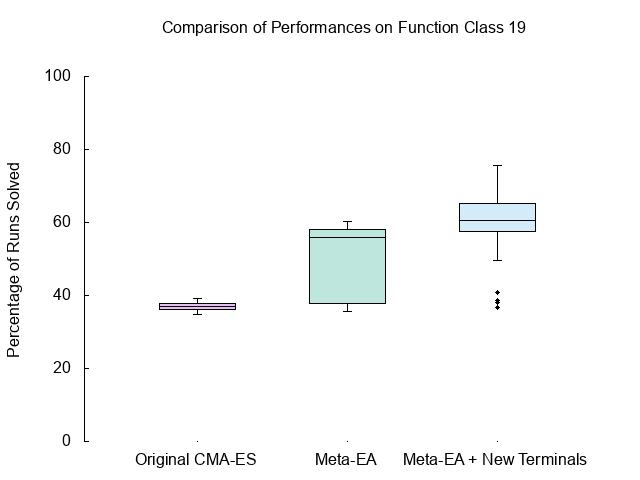
\includegraphics[width=0.45\textwidth]{terminalPerformanceComp}
	\caption{Comparing CMA-ES performance for base, meta-EA evolved, and expanded terminal meta-EA evolved cases.}
	\label{fig:terminalPerformanceComp}
\end{figure}

\section{Search Methodology}
\label{Search Methodology}

We use a meta-EA to develop the selection functions, treating each complete selection function as a member of a higher-order population. After generating an initial pool of randomly constructed selection functions, the quality of each complete selection function is determined, and well-performing selection functions are chosen to recombine and mutate into new candidate selection functions. The size of the trees is constrained using parsimony pressure.

We target the CMA-ES algorithm for improvement, evolving a new selection function for the mean-update algorithm. The quality of each selection function is determined by running CMA-ES on a suite of static training instances selected from the Comparing Continuous Optimizers (COCO) platform used for the GECCO Workshops on Real-Parameter Black-Box Optimization Benchmarking~\citep{cocobbob}. Each of the 24 noiseless benchmark problem classes in COCO is offered in multiple dimensions, and for each dimension, multiple problem instances are present. We select 11 of the 24 problem classes and use dimensions 2, 3, 5, and 10. The problem classes were selected by running unmodified CMA-ES on each of the 24 problem classes, selecting those where it failed to solve some dimension $D \leq 10$ on at least half of the trial runs. For each class and dimension, we set aside some instances to test for generalization.

A second experiment investigated the effects of expanding the terminal set. New terminals tested were a genome's Euclidean distance to the best genome found during the run, generations since the last improvement in fitness, and the last generation's average fitness. The effects of adding and removing terminals were tested on function classes 3, 16, 19, and 21 with $D=2$. These were the function classes where neither the modified nor the unmodified CMA-ES reached a 100\% success rate. 

\section{Results and Discussion}
\label{Results}

For function classes 4 and 19, the success rate of CMA-ES increased by 20-30\% when modified with the evolved selection function at $D=2$, but performed similarly to unmodified CMA-ES at other dimensionalities. For function classes 20 and 21, a performance increase is seen on dimensionalities $D=2, 3,$ and $5$, but not $D=10$. For function classes 6 and 12, performance is similar for $D=2, 3,$ and $5$, but for $D=10$, there is a significant performance increase: on function class 6, the success rate increased from 0\% to around 96\%, and on function class 12, the success rate increased from 18-67\%, varying across function instances, to 100\% for all function instances. For the remaining function classes, there was no major difference in success rate. These cases involved highly multimodal functions, and CMA-ES likely requires some other improvement to better traverse the global structures of these functions. $F=21$, $D=10$ is the one case where CMA-ES performed worse than unmodified CMA-ES. This effect is likely due to overspecialization to the set of training instances. 

In the second experiment, including the terminal for Euclidean distance to the best-found genome resulted in a significant boost in performance, but only if Euclidean distance to the average genome was also included. Function class 3's success rate went from 32.09\% to 58.51\%, function class 16's from 65.57\% to 68.91\%, function class 19's from 50.21\% to 59.20\%, and function class 23's from 71.56\% to 86.07\%. The addition of the two terminals did not significantly increase the number of generations needed for the meta-EA. The ending performances on function class 19 are summarized in Figure~\ref{fig:terminalPerformanceComp}.

The benefit of the new terminals is clear from the four function classes tested. The fact that the two Euclidean distance terminals only boost performance significantly when together suggests that the benefit of adding terminals can be highly dependant on the other terminals in the terminal set. Further investigation into new terminals could lead to significant improvements in the modified CMAE-ES's performance.

\section{Conclusions}
\label{Conclusion}
We hypothesized that a search through the space of selection functions could improve the performance of an EA on a particular problem class by discovering a specialized selection function. We developed a representation of selection functions that utilize a GP-Tree and selection method and used a meta-EA to search through the space of selection functions in this representation. 

We have shown that it is possible to generate new selection functions and tune the performance of an EA to outperform conventional strategies on a selected benchmark problem significantly. We have also shown that this performance increase will generalize to similar problems in the same problem class. Thus, if one expects to run the same EA on the same problem class many times, one might gain a performance increase by doing \textit{a priori} calculation to develop a specialized selection algorithm, which would then enable an EA to perform better on instances of that problem class. However, we have also shown that, for certain functions, replacing only the selection function may not yield significant performance improvements, depending on the particular EA and the function being solved. Careful consideration must be given to determine what the effect of tuning the selection scheme will be on the performance of a given EA and whether such tuning will result in a substantial performance increase. 

\bibliography{eppsea_GECCO2019_bibliography}
\bibliographystyle{plain}
\end{document}
